% Chapter Template


\chapter{Results and Discussion}

\label{Chapter6:Results}

%----------------------------------------------------------------------------------------
% Transfer learning
% effect of loss function
% effect of camera intrinsic 
% effect of Hyper parameter
% Effect of recreating holes.. 
 
 
%----------------------------------------------------------------------------------------
In this chapter we have evaluated your system and presented a comparative results  based on different experimental setup discussed in section \ref{Chapter5:Methodology}. We have categorized our experiments into 3 different sections as shown in the table below \ref{table:Results_main} to investigate in three difference area. The table \ref{table:Results_main} lists all the experiments carried out for this study on depth estimation. We have 3 accuracy values based on different threshold namely (a1, a2, and a2) and two error metrics namely root mean square error (rms) and log\_10 error as mentioned in section. Experiments \textbf{E1} and \textbf{E2} where performed to understand the importance of structural dependency of depth maps and to test our proposed model against the state of the art system. In experiments \textbf{E3} and \textbf{E4} we validate the influence of different camera intrinsic properties over data from structure sensor, by this we can also see the influence of transfer learning even when trained on different dataset with different feature properties. Experiments \textbf{E5} and \textbf{E6} was carried out to study behaviour of probabilistic distribution over the invalid pixel which we call it as holes, this leads us to answer the question of efficient way for depth estimation.
 
 Test data: 271 image
 Train
 
% Please add the following required packages to your document preamble:
% \usepackage{multirow}
\begin{table}[b]
\begin{tabular}{p{0.05\linewidth}p{0.3\linewidth}p{0.1\linewidth}p{0.1\linewidth}p{0.1\linewidth}p{0.1\linewidth}p{0.1\linewidth}}
\hline
\textbf{\#} & \textbf{Model} & \multicolumn{3}{l}{\textbf{Accuracy}} & \multicolumn{2}{l}{\textbf{Error}} \\ \cline{3-7} 
                    &                        & a1       & a2       & a3      & RMSE         & log\_10      \\ \hline
\multicolumn{7}{l}{\texttt{Influence of Structural Characteristics}}                                            \\ \hline
\textbf{E1}                  &  \textbf{A1}  & 0.22         & 0.43          &  0.61       & 0.34            &   0.001           \\ \hline
\textbf{E2}                  & \textbf{A2}  &    0.60  & 0.859 & 0.93       &   0.19          &0.11              \\ \hline
\multicolumn{7}{l}{\texttt{Influence Of Transfer Learning}}                                                                   \\ \hline
\textbf{E3}                  & \textbf{A2\_Holes}              & 0.39   & 0.58   & 0.65  & 0.27      & 1.70       \\ \hline
\textbf{E4}                  & \textbf{A2\_Holes} (Retrained) & 0.33   & 0.55   & 0.63  & 0.34      & 1.78       \\ \hline
\multicolumn{7}{l}{\texttt{Holes Regeneration}}                                                       \\ \hline
\textbf{E5}                  & \textbf{A2\_NoHoles}            & 0.98   & 0.98   & 0.98  & 0.10       & 0.18        \\ \hline
\textbf{E6}                  & \textbf{A2\_Holes}              & 0.39   & 0.58   & 0.65  & 0.27      & 1.70       \\ \hline
\end{tabular}

\caption{This table list all the depth estimation experiment on Structure dataset. These experiments are grouped in to 3 catogories.}
\label{table:Results_main}
\end{table}


\section{Influence of Structural Characteristics}
\label{Chapter6:Influence_Structural_Char}
In this section we have investigated the Influence of Structural Characteristics of a pre-trained network.  As discribed in the section \ref{Chapter5:Methodology} we designed \textbf{A1} a simple U-Net to test against a pre-trained network by ImageNet with DenseNet configuration \textbf{A2}. 
 
 
 
 Hence, we have a robust architecture for depth map estimation which intern helps for a better 
 
 \begin{figure}
\settoheight{\tempdima}{\includegraphics[width=.32\linewidth]{example-image-a}}%
\centering\begin{tabular}{@{}c@{ }c@{ }c@{ }c@{}}
&\textbf{RGB} & \textbf{Truth} & \textbf{Predticted} \\
\rowname{E1 (a)}&
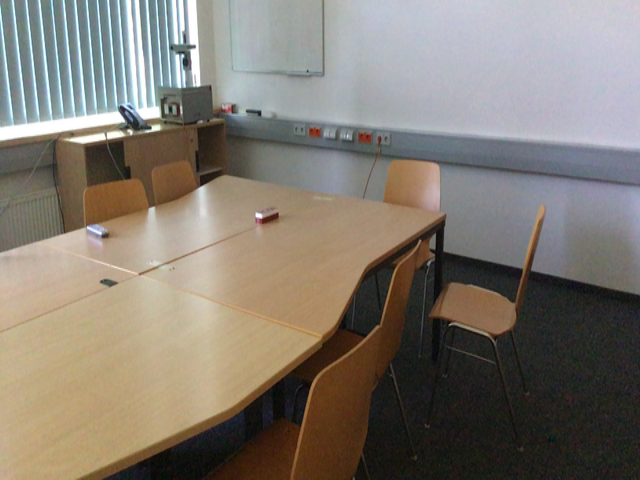
\includegraphics[width=.3\linewidth]{Figures/results/s1_a1/u0RAW_RGB.png}&
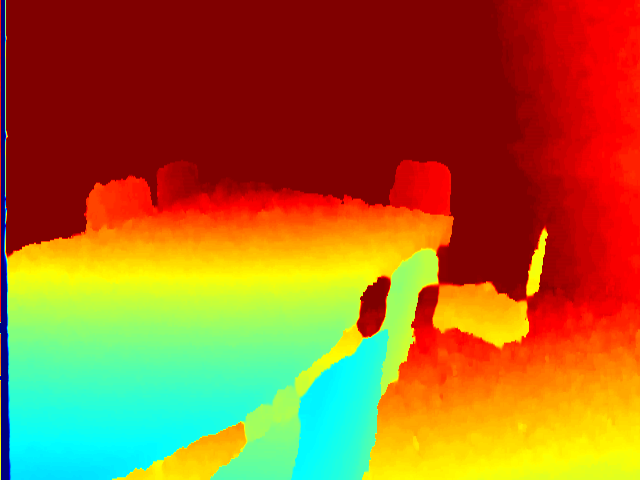
\includegraphics[width=.3\linewidth]{Figures/results/s1_a1/u0Truth.png}&
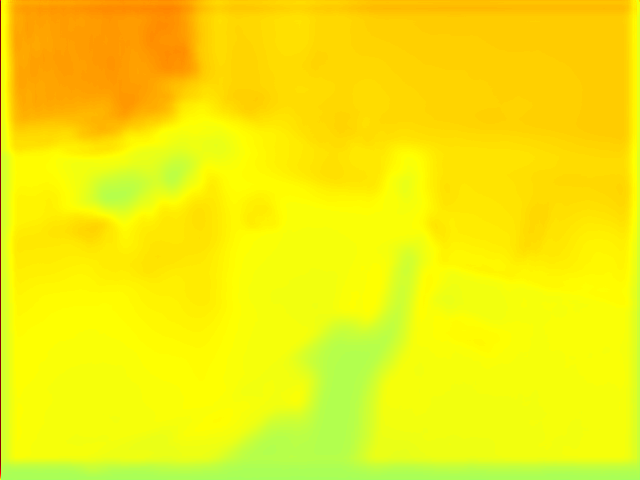
\includegraphics[width=.3\linewidth]{Figures/results/s1_a1/u0Predicted.png}\\[-1ex]
\rowname{E2 (b)}&
\includegraphics[width=.3\linewidth]{Figures/results/s1_a1/0RAW_RGB.png}&
\includegraphics[width=.3\linewidth]{Figures/results/s1_a1/0Truth.png}&
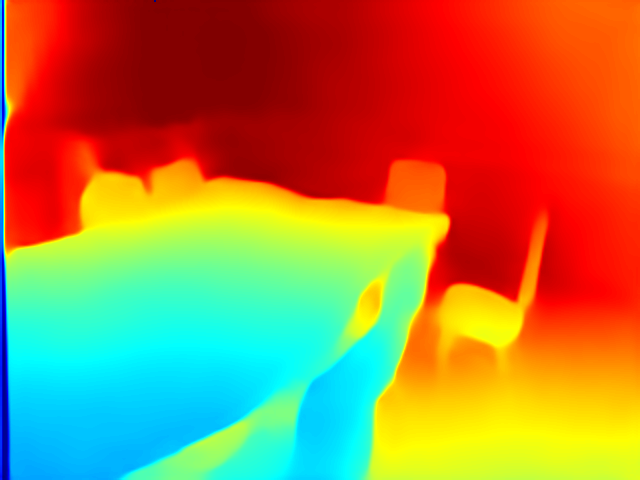
\includegraphics[width=.3\linewidth]{Figures/results/s1_a1/0Predicted.png}\\[-1ex]
\end{tabular}
\caption{\textbf{Influence of Structural Characteristics:} All the \textbf{E3} methods are in different  }%
\label{figure1}
\end{figure}


 

 \section{Influence Of Transfer Learning}
 \label{Chapter6:Transfer_Learning}
 
 
 \begin{figure}
\settoheight{\tempdima}{\includegraphics[width=.32\linewidth]{example-image-a}}%
\centering\begin{tabular}{@{}c@{ }c@{ }c@{ }c@{}}
&\textbf{RGB} & \textbf{Truth} & \textbf{Predticted} \\
\rowname{E4 (a)}&
\includegraphics[width=.3\linewidth]{Figures/results/s2_Holes/0RAW_RGB.png}&
\includegraphics[width=.3\linewidth]{Figures/results/s2_Holes/0Truth.png}&
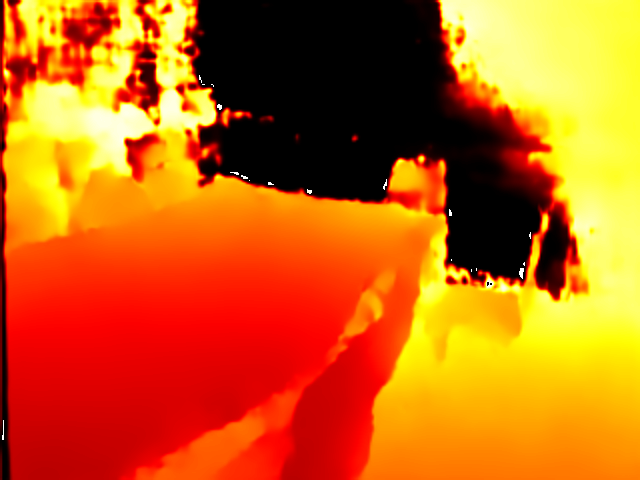
\includegraphics[width=.3\linewidth]{Figures/results/s2_Holes/0Predicted.png}\\[-1ex]
&\mycaption{} & \mycaption{} & \mycaption{} \\
\rowname{E4 (a)}&
\includegraphics[width=.3\linewidth]{Figures/results/s2_Holes/1RAW_RGB.png}&
\includegraphics[width=.3\linewidth]{Figures/results/s2_Holes/1Truth.png}&
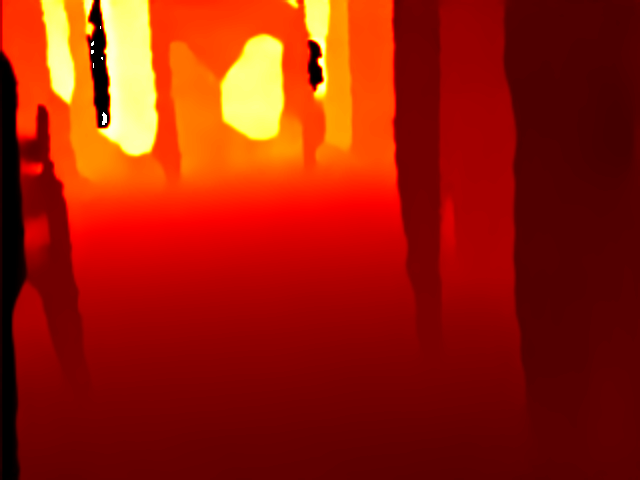
\includegraphics[width=.3\linewidth]{Figures/results/s2_Holes/1Predicted.png}\\[-1ex]
&\mycaption{} & \mycaption{} & \mycaption{} \\
\rowname{E4 (a)}&
\includegraphics[width=.3\linewidth]{Figures/results/s2_Holes/2RAW_RGB.png}&
\includegraphics[width=.3\linewidth]{Figures/results/s2_Holes/2Truth.png}&
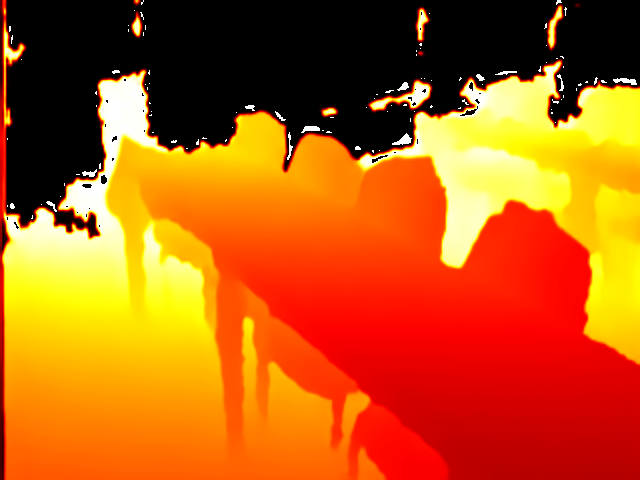
\includegraphics[width=.3\linewidth]{Figures/results/s2_Holes/2Predicted.png}\\[-1ex]
&\mycaption{} & \mycaption{} & \mycaption{} \\
\rowname{E3 (a)}&
\includegraphics[width=.3\linewidth]{Figures/results/s3_noNyu/0RAW_RGB.png}&
\includegraphics[width=.3\linewidth]{Figures/results/s3_noNyu/0Truth.png}&
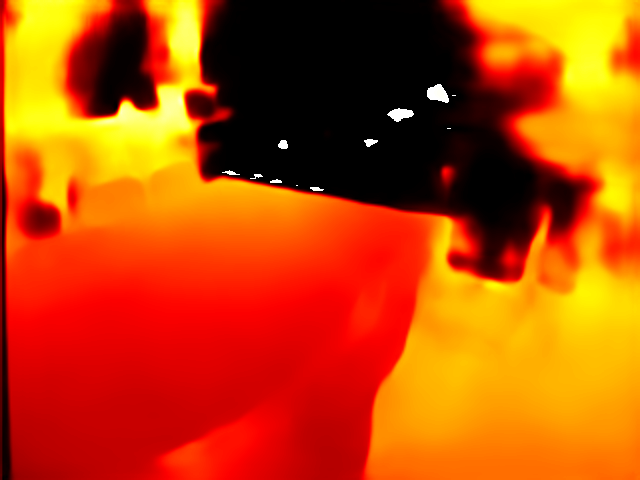
\includegraphics[width=.3\linewidth]{Figures/results/s3_noNyu/0Predicted.png}\\[-1ex]
&\mycaption{} & \mycaption{} & \mycaption{} \\
\rowname{E3 (a)}&
\includegraphics[width=.3\linewidth]{Figures/results/s3_noNyu/1RAW_RGB.png}&
\includegraphics[width=.3\linewidth]{Figures/results/s3_noNyu/1Truth.png}&
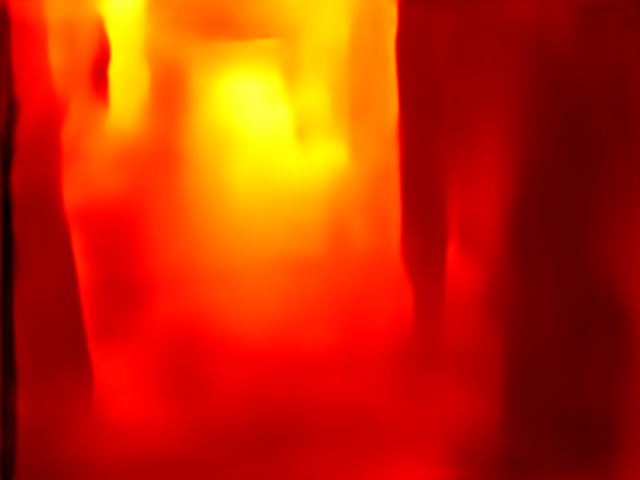
\includegraphics[width=.3\linewidth]{Figures/results/s3_noNyu/1Predicted.png}\\[-1ex]
&\mycaption{} & \mycaption{} & \mycaption{} \\
\rowname{E3 (a)}&
\includegraphics[width=.3\linewidth]{Figures/results/s3_noNyu/2RAW_RGB.png}&
\includegraphics[width=.3\linewidth]{Figures/results/s3_noNyu/2Truth.png}&
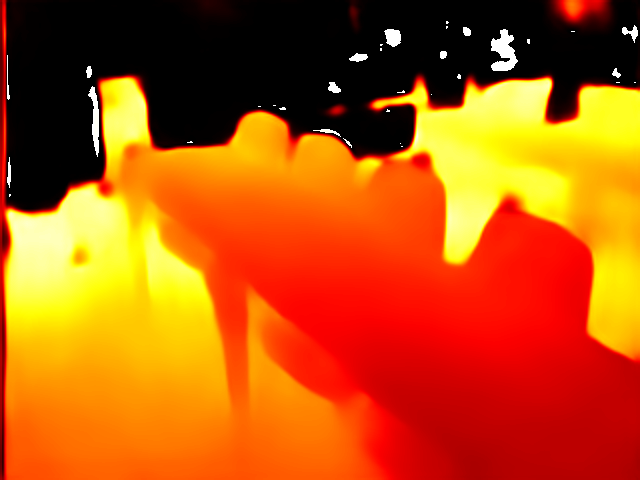
\includegraphics[width=.3\linewidth]{Figures/results/s3_noNyu/2Predicted.png}\\[-1ex]
&\mycaption{} & \mycaption{} & \mycaption{} \\
\end{tabular}
\caption{\textbf{Investigation on hole regeneration method:} All the \textbf{E3} methods are in different  }%
\label{figure1}
\end{figure}









 \section{Hole Regeneration Method}
 \label{Chapter6:Hole_Regeneration}
Further more to improve the results for estimation of depth maps for 3D reconstruction as our application of this work, we study the importance/influence of effects of a probabilistic distribution while regenerating holes. As described in section \ref{Chapter4:Dataset}, in order to have a holes recreated we mapped all the dead value or no pixel region as zero pixel. Therefore we have two methods of pre-possessing carried out with two different input feature type, one with holes and another without holes. We tested the performance of \textbf{A2\_Holes} against the \textbf{A2\_NoHoles} models. For both the experiments we used \textbf{A2} architecture.  In Fig. \ref{fig:results_S2} (a) - (c) we see that there a good reconstruction of the depth map were all the holes were interpolated to its neighboring pixel.  Fig. \ref{fig:results_S2} (d) - (f)  corresponds to the model with the holes as a input to the network. As we see in Fig \ref{fig:results_S2}, we compare \textbf{E5} and \textbf{E6}. We have used two different color maps for \textbf{E5} and \textbf{E6}. This is because in \textbf{E4} we wanted to highlight the difference between holes which were mapped to zero and the closest region in an image. 

From the table \ref{table:Results_main} we notice that the on an average the model \textbf{E3 (A2\_NoHoles)} performs better. When RMSE is taken into consideration we can clearly see that \textbf{E3 (A2\_NoHoles)} performs better with the RMSE of \textbf{0.10} which is \textbf{0.17} lower than the \textbf{E4 (A2\_Holes)} with RMSE of \textbf{0.27}. And when we notice our accuracy a1, a2 and a3 we see the similar results when compared. But when notice in the Fig. \ref{fig:results_S2} (d) - (f) we have visually good prediction. when investigated further why such hugh difference in the accuracy and error we found out the error lies in the object boundaries. As we see in the fig () there is a interpolation intermediate pixel from the zero value (holes which are mapped as zeros) till the actual depth. This effect is cause because of the probabilistic distribution method of neural network characteristic. We strongly this is one of there main factors contributing to the difference in the error and accuracy between \textbf{E5} and \textbf{E6}. Now that we understand why such effects can be seen for the generation of holes, it is very important us to answer if such approach is beneficial or not. Given such a problem of linear \notice{interpolating prediction} one possible solotion can be given by some post-filtering or post processing methods but the idea for the case of this study is to provide end to end approch as much as possible thereby exploiting the potential of the neural network. 

Therefore we see that given an input with holes the model can learn the holes from the given monocular input. But it results into \notice{interpolatin prediction} which we believe makes the 3D reconstruction of a scene more difficult and demands further post processing techniques. This leads us to an conclusion that interpolating of pixel is a better approach than making the network learn to predict holes. In addition to this, one of the other motivation to try this approach was to eliminate the wall effect of depth maps  for the pixel farther than the distance limit, one approach for this solution could be taking a threshold just before the highest pixels. This solves the problem of having wall in out 3D reconstruction scene.

In summary, we believe that the comparing the two different input representation, \textbf{A2\_NoHoles} approach where the holes are interpolated with its neighboring pixels is beneficial.





\begin{figure} 
\settoheight{\tempdima}{\includegraphics[width=.32\linewidth]{example-image-a}}%
\centering\begin{tabular}{@{}c@{ }c@{ }c@{ }c@{}}
&\textbf{RGB} & \textbf{Truth} & \textbf{Predticted} \\
\rowname{E3 (a)}&
\includegraphics[width=.3\linewidth]{Figures/results/s2_NoHoles/0RAW_RGB.png}&
\includegraphics[width=.3\linewidth]{Figures/results/s2_NoHoles/0Truth.png}&
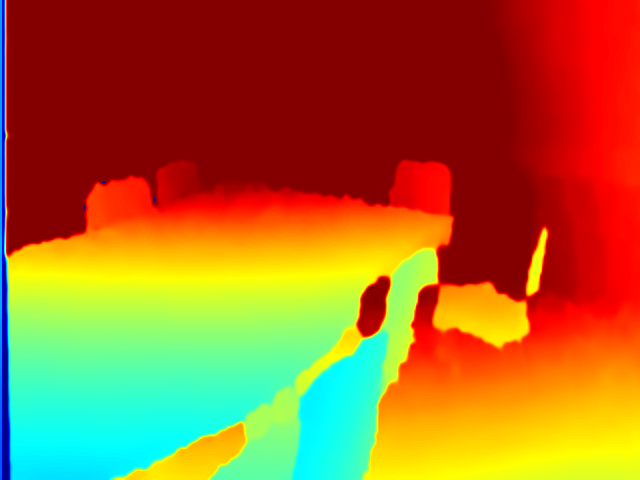
\includegraphics[width=.3\linewidth]{Figures/results/s2_NoHoles/0Predicted.png}\\[-1ex]
\rowname{E3 (b)}&
\includegraphics[width=.3\linewidth]{Figures/results/s2_NoHoles/1RAW_RGB.png}&
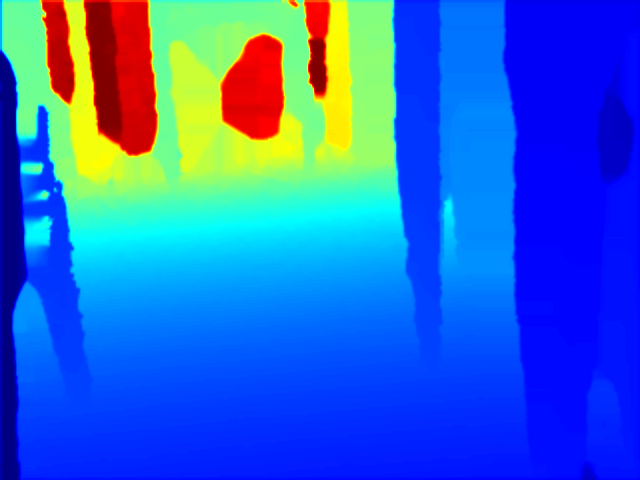
\includegraphics[width=.3\linewidth]{Figures/results/s2_NoHoles/1Truth.png}&
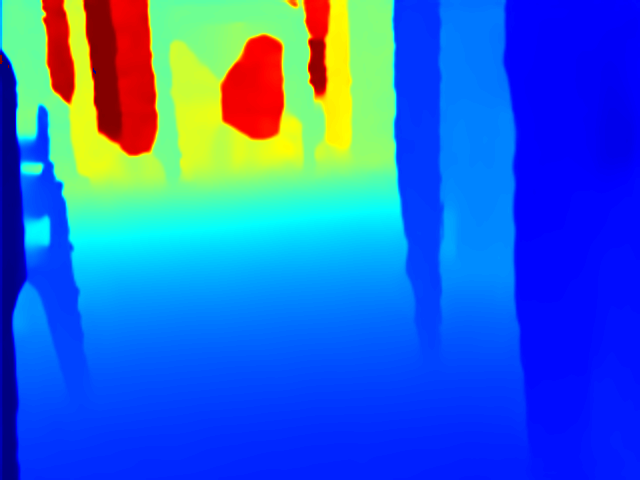
\includegraphics[width=.3\linewidth]{Figures/results/s2_NoHoles/1Predicted.png}\\[-1ex]
\rowname{E3 (c)}&
\includegraphics[width=.3\linewidth]{Figures/results/s2_NoHoles/2RAW_RGB.png}&
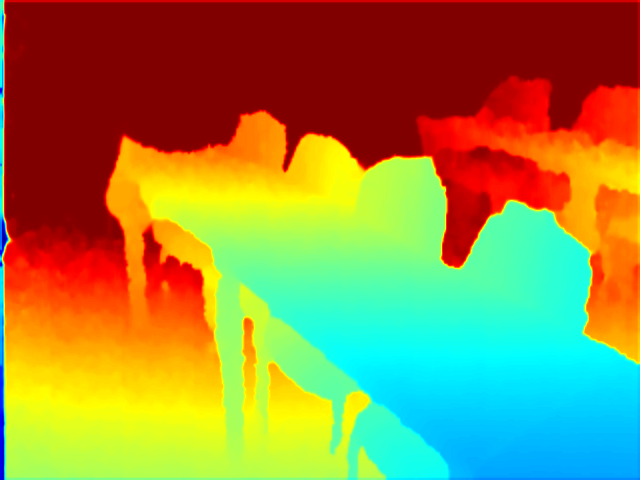
\includegraphics[width=.3\linewidth]{Figures/results/s2_NoHoles/2Truth.png}&
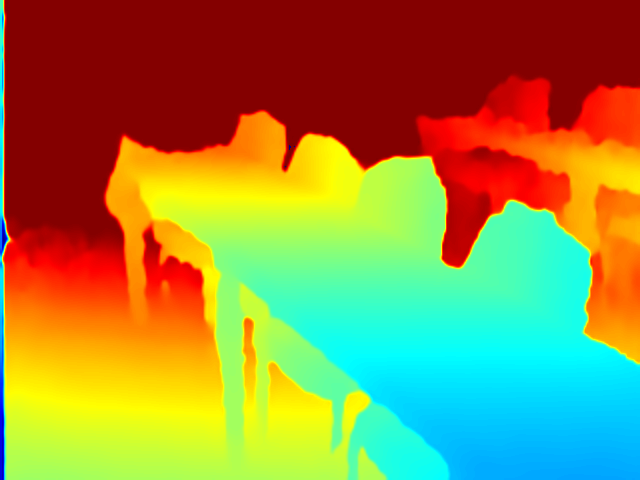
\includegraphics[width=.3\linewidth]{Figures/results/s2_NoHoles/2Predicted.png}\\[-1ex]
\rowname{E4 (d)}&
\includegraphics[width=.3\linewidth]{Figures/results/s2_Holes/0RAW_RGB.png}&
\includegraphics[width=.3\linewidth]{Figures/results/s2_Holes/0Truth.png}&
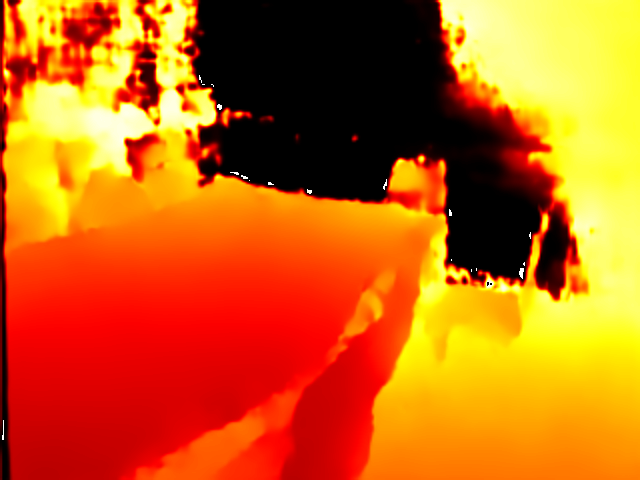
\includegraphics[width=.3\linewidth]{Figures/results/s2_Holes/0Predicted.png}\\[-1ex]
\rowname{E4 (e)}&
\includegraphics[width=.3\linewidth]{Figures/results/s2_Holes/1RAW_RGB.png}&
\includegraphics[width=.3\linewidth]{Figures/results/s2_Holes/1Truth.png}&
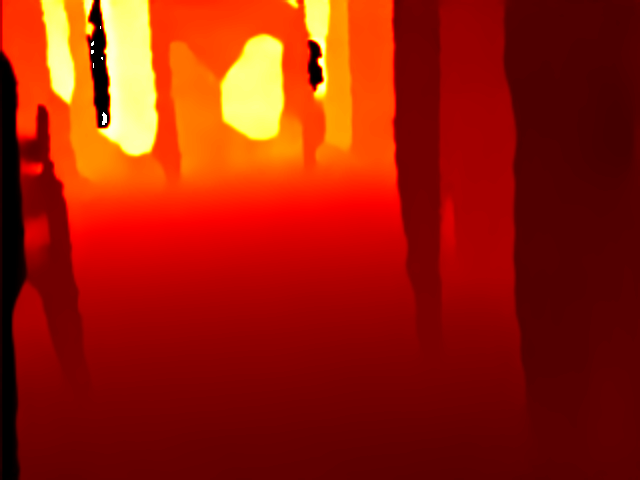
\includegraphics[width=.3\linewidth]{Figures/results/s2_Holes/1Predicted.png}\\[-1ex]
\rowname{E4 (f)}&
\includegraphics[width=.3\linewidth]{Figures/results/s2_Holes/2RAW_RGB.png}&
\includegraphics[width=.3\linewidth]{Figures/results/s2_Holes/2Truth.png}&
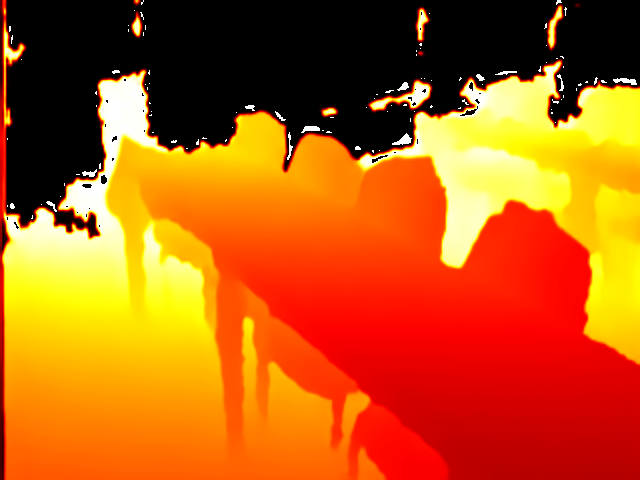
\includegraphics[width=.3\linewidth]{Figures/results/s2_Holes/2Predicted.png}\\[-1ex]
\end{tabular}
\caption{\textbf{Investigation on hole regeneration method:} All the \textbf{E3} methods are in different  }%
\label{fig:results_S2}
\end{figure}





 
 
 

In order to have a holes recreated we mapped all the dead value or no pixel region as zero pixel as described in section \ref{Chapter4:Dataset}. We tested \ this against the 